%!TEX root = ../template.tex
%%%%%%%%%%%%%%%%%%%%%%%%%%%%%%%%%%%%%%%%%%%%%%%%%%%%%%%%%%%%%%%%%%%
%% chapter4.tex
%% NOVA thesis document file
%%
%% Chapter with introduction
%%%%%%%%%%%%%%%%%%%%%%%%%%%%%%%%%%%%%%%%%%%%%%%%%%%%%%%%%%%%%%%%%%%

\typeout{NT FILE chapter5.tex}%

\chapter{Spectral analysis}

Now that the theoretical spectrum has been simulated, it is time to analyze the evolution of the emission lines with the change in the beam energy. Results will then be compared with a recent work by Y. Ito ?? where measurements of Copper's x-ray transitions were taken for



\section{Result analysis}

For peak analysis, fits were performed for each beam energy using a similar proceeding as in ??\todo{cite}, where two asymmetric Lorentzian profiles were employed.

In order to compute the asymmetrical Lorentzian profile, an asymmetry parameter, $\alpha$, was incorporated:

\begin{equation}
    L_{\text{assim}}(E-E_{i,f},\Gamma_{i,f},\sigma,\alpha)=\frac{I_{i,f}}{2\pi}\frac{\Gamma_{i,f}}{\qty(\frac{E-E_{i_f}}{\alpha\cdot \text{sign}\qty(E-E_{i_f})+1})^2+\qty(\frac{\Gamma_{i,f}}{2})^2}
\end{equation}

The influence of the calculated excitations will now be noted in the obtained parameters, resulting, in some cases, in extremely non-linear parameter progression.
\subsection{Centroid energy}

For the $K_{\alpha_1}$ line, a very noticeable energy shift of around $0.5\ \si{\electronvolt}$ is observed at the second $4p$ resonance-dominated zone. Once again, poor numerical convergence may be the cause of this.

On the case of the $K_{\alpha_2}$ line, the results are less anomalous, as there is a steady rise of the centroid energy, with the influence of different excited states being noted as sudden bumps and lows.

Both spectral line energies are lower on the pre-ionization region, and saturate for beam energy values over the K edge, with $K_{\alpha_1}$ possessing an energy of $\qty(8047.093\pm0.002)\ \si{\electronvolt}$ and $K_{\alpha_2}$ of $\qty(8026.683\pm0.004)\ \si{\electronvolt}$   at $E_{\text{beam}}=8970\ \si{\electronvolt}$, and rising to $\qty(8047.12926 \pm 0.00001)\ \si{\electronvolt}$ and $\qty(8027.05247 \pm 0.00002)\ \si{\electronvolt}$, respectively, for the post-ionization region.

Figure~\ref{fig:centroid} contains the whole evolution of the centroid parameters.

\begin{figure}[h!]
    \centering
    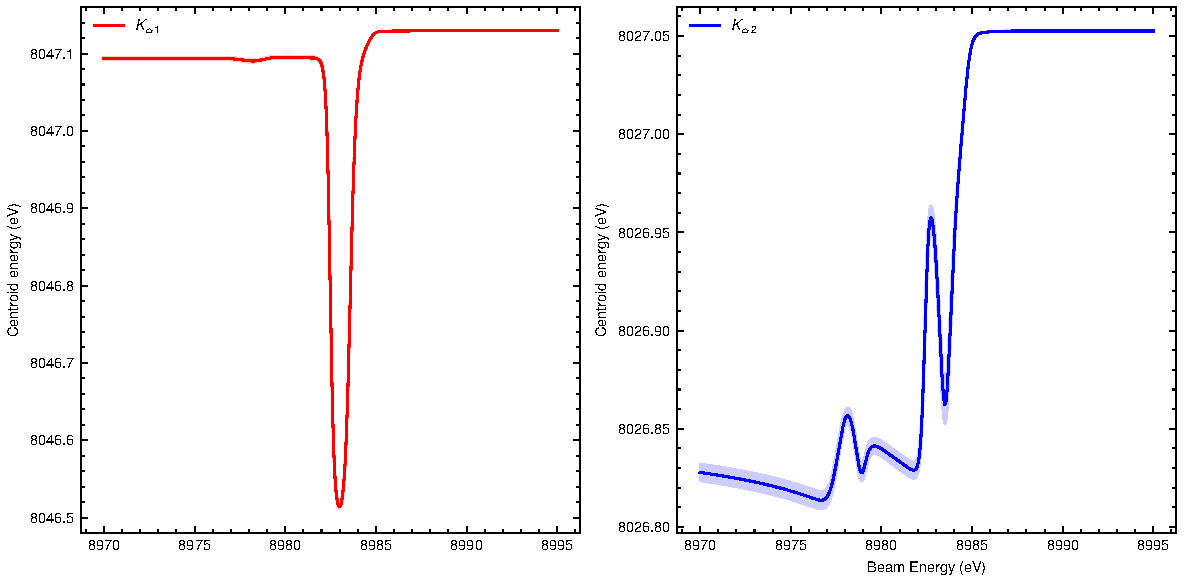
\includegraphics[width=\linewidth]{Chapters/Figures/Chapter5/assym_centroids.pdf}
    \caption{Evolution of centroid parameter as a function of the beam energy.}\label{fig:centroid}
\end{figure}

\subsection{Energy width}

As for the energy widths, both $K_{\alpha}$ transitions present a theoretical value of around $2.2\ \si{\electronvolt}$ for the post-ionization region ($\qty(2.25137\pm 0.00003)\ \si{\electronvolt}$ and $\qty(2.21834\pm 0.00006)\ \si{\electronvolt}$ for $K_{\alpha_1}$ and $K_{\alpha_2}$, respectively). Both present higher values than these for the excitation-dominated region, with $K_{\alpha_2}$ being wider than $K_{\alpha_1}$. The ratio between these two widths steadily increases, while making apparent the influeces


 



\section{Comparison with experimental results}